\documentclass[12pt,onecolumn,journal,draftclsnofoot]{IEEEtran}
\usepackage{amsmath,amssymb,amsthm}
\usepackage{etoolbox}
\usepackage[mathlines]{lineno}
\usepackage{algorithm}
\usepackage{algpseudocode}
\usepackage{graphicx}
\usepackage[colorlinks=true,linkcolor=blue,citecolor=blue,urlcolor=blue]{hyperref}
\usepackage{xcolor}
\usepackage{draftwatermark}
\SetWatermarkText{Working draft: Jun 10, 2026}
\SetWatermarkFontSize{30pt}
\SetWatermarkAngle{55}
\SetWatermarkLightness{0.85}

% number displayed equations' lines (amsmath makes \[ \] = equation*)
\newcommand*\linenomathpatchAMS[1]{%
  \expandafter\pretocmd\csname #1\endcsname {\linenomathAMS}{}{}%
  \expandafter\pretocmd\csname #1*\endcsname{\linenomathAMS}{}{}%
  \expandafter\apptocmd\csname end#1\endcsname {\endlinenomath}{}{}%
  \expandafter\apptocmd\csname end#1*\endcsname{\endlinenomath}{}{}%
}
\expandafter\ifx\csname linenomathWithnumbers\endcsname\relax
  \let\linenomathAMS\linenomath
\else
  \let\linenomathAMS\linenomathWithnumbers
\fi
\linenomathpatchAMS{equation}

\newtheorem{theorem}{Theorem}
\newtheorem{proposition}{Proposition}
\newtheorem{lemma}{Lemma}
\newtheorem{corollary}{Corollary}
\newtheorem{definition}{Definition}
\newtheorem{assumption}{Assumption}
\newtheorem{remark}{Remark}

\newcommand{\R}{\mathbb{R}}
\newcommand{\Sym}{\mathbb{S}}
\newcommand{\X}{\mathcal{X}}
\newcommand{\D}{\mathcal{D}}
\newcommand{\lmax}{\lambda_{\max}}
\providecommand{\tr}{}
\renewcommand{\tr}{\operatorname{tr}}
\newcommand{\todo}[1]{\textcolor{red}{[VR: #1]}}

\title{Neurosymbolic Synthesis of Contraction Certificates}

\author{Victor~M.~Preciado,~\IEEEmembership{Senior~Member,~IEEE}%
\thanks{V.~M.~Preciado is with the Department of Electrical and Systems
Engineering and the Department of Computer and Information Science,
University of Pennsylvania, Philadelphia, PA 19104 USA
(e-mail: preciado@seas.upenn.edu).}%
\thanks{Working draft of June 10, 2026. Not yet submitted.}}

\markboth{Working draft, June 10, 2026}{Preciado: Neurosymbolic Synthesis of Contraction Certificates}

\begin{document}
\maketitle
\linenumbers

\begin{abstract}
We propose a neurosymbolic framework for synthesizing contraction metrics with formal guarantees: a neural learner proposes a candidate metric, a sound symbolic oracle either certifies the contraction condition over a compact domain or returns counterexamples, and the counterexamples drive retraining. Counterexample-guided inductive synthesis (CEGIS) of this kind is established for Lyapunov and barrier certificates, but the contraction case has remained open because the certificate condition is a parametrized matrix inequality rather than a scalar one. We close the loop and analyze it. We prove that the certifiability of a candidate metric is invariant under positive scaling, which implies that margin-driven learners operating on the raw contraction condition can diverge by inflating the metric's scale, and that a trace-normalized test function removes the degeneracy. We characterize a stall mode of fixed-margin learners as a non-certified fixed point of the loop. We then show that verification slack converts into guarantees: a metric certified with uniform margin $\eta$ yields contraction at a rate improved by $\eta/(2b)$, and when the dynamics are themselves learned with residual bounds $(\delta_0, \delta_1)$, the same slack absorbs the model error and yields an explicit contraction rate for the true system. Computational experiments on a benchmark with a known state-dependent metric illustrate all three phenomena: the stall, the scale chase, and certification by the normalized margin-coupled loop in one retraining round, together with a quantification of the grid oracle's exponential cost in the state dimension. The controlled case via control contraction metrics is the subject of a sequel.
\end{abstract}

\begin{IEEEkeywords}
Contraction theory, counterexample-guided inductive synthesis, formal verification,
learning-based control, neurosymbolic AI.
\end{IEEEkeywords}

\section{Introduction}

Learning-based methods now propose models and controllers for nonlinear systems faster than formal methods can certify them. The certificate-learning literature addresses this gap by training neural networks to represent stability and safety certificates, then verifying the result \cite{dawson2023}. For Lyapunov and barrier functions the mature architecture is neurosymbolic: a neural learner proposes a candidate, a sound symbolic verifier (an SMT solver, an interval engine, or a neural network verifier) either certifies it over a whole domain or returns counterexamples, and the counterexamples augment the training set. This counterexample-guided inductive synthesis (CEGIS) loop \cite{solar2006} is implemented end to end in tools such as Fossil 2.0 \cite{edwards2024} and has been used to certify deep reinforcement learning controllers \cite{mandal2024,chang2019,abate2021}.

Contraction certificates have not received the same treatment. Contraction theory \cite{lohmiller1998,manchester2017,tsukamoto2021tutorial} certifies incremental stability, the exponential convergence of trajectories toward one another, through a Riemannian metric whose induced differential dynamics decay uniformly. The payoff exceeds that of point-stability certificates: contraction yields tracking guarantees, composes across interconnections, and extends to stochastic settings. Neural representations of contraction metrics exist \cite{tsukamoto2021ncm,sun2021}, and sound a posteriori verification schemes for them exist, based on Lipschitz margins over grids \cite{sun2021} or interval matrix analysis \cite{anonymous2026}. What does not exist, to our knowledge, is the loop: no published method feeds contraction verification failures back into metric training, and no work places contraction analysis within the neurosymbolic paradigm.

This paper closes the loop and shows that doing so is not a transcription exercise. The matrix structure of the contraction condition introduces failure modes with no Lyapunov analogue, and their analysis produces the paper's main results. Our contributions are as follows. First, we formalize neurosymbolic synthesis of contraction metrics and prove soundness of the grid-based verification oracle and of the resulting CEGIS loop, which we call CEGIS-C (Section~\ref{sec:framework}). Second, we prove a scale-invariance lemma: positive scaling of the metric scales the contraction condition, its worst value, and its Lipschitz constant identically, so certifiability depends only on the metric's shape. The lemma implies that a margin-driven learner operating on the raw condition can satisfy every training requirement by inflating the metric's scale while making no progress toward certification, and it dictates the remedy, a trace-normalized test function (Section~\ref{sec:results}). Third, we characterize the stall mode of fixed-margin learners as a non-certified fixed point of the loop (Section~\ref{sec:results}). Fourth, we prove two slack-to-guarantee theorems: certification with uniform margin $\eta$ improves the contraction rate by $\eta/(2b)$, and when the vector field is itself a learned surrogate with residual bounds, the same margin absorbs the model error and yields an explicit contraction rate for the true dynamics (Section~\ref{sec:results}). Fifth, we illustrate every phenomenon computationally on a benchmark with a known state-dependent metric, and we quantify the exponential cost of the grid oracle in the state dimension, locating the current certification frontier (Section~\ref{sec:experiments}).

We restrict attention to autonomous contraction. The controlled case, control contraction metrics \cite{manchester2017}, involves the dual metric $W = M^{-1}$ and additional structural conditions; carrying the present framework to that setting is the subject of a sequel.

\section{Preliminaries}
\label{sec:prelim}

Consider the system
\begin{equation}
\dot{x} = f(x), \qquad x \in \X \subset \R^n,
\label{eq:sys}
\end{equation}
with $f$ continuously differentiable and $\X$ compact. Write $A(x) = \partial f/\partial x\,(x)$. A continuously differentiable $M : \X \to \Sym^n_{++}$ with
\begin{equation}
a I \preceq M(x) \preceq b I \quad \text{on } \X, \qquad 0 < a \le b,
\label{eq:bounds}
\end{equation}
is a contraction metric with rate $\lambda > 0$ on $\X$ if
\begin{equation}
C(x) \;:=\; \dot{M}(x) + A(x)^\top M(x) + M(x) A(x) + 2\lambda M(x) \;\preceq\; 0
\qquad \text{for all } x \in \X,
\label{eq:contraction}
\end{equation}
where $\dot{M}(x) = \sum_{i=1}^{n} \frac{\partial M}{\partial x_i}(x) f_i(x)$. If \eqref{eq:contraction} holds, then for any two trajectories remaining in $\X$ the virtual displacement satisfies $\|\delta x(t)\| \le \sqrt{b/a}\, e^{-\lambda t} \|\delta x(0)\|$ \cite{lohmiller1998}.

The candidate metric is a parametric family $M_\theta$, $\theta \in \Theta \subseteq \R^p$, with symmetry and the bounds \eqref{eq:bounds} enforced by construction, for instance the Cholesky-type parametrization
\begin{equation}
M_\theta(x) = \alpha I + L_\theta(x)^\top L_\theta(x), \qquad \alpha > 0,
\label{eq:class}
\end{equation}
with $L_\theta(x)$ lower triangular and its entries given by linear combinations, with coefficients $\theta$, of fixed features of $x$. The lower bound $a = \alpha$ holds for every $\theta$; the upper bound $b$ follows from bounding $\|L_\theta\|$ on the compact $\X$. We write $C_\theta(x)$ for the matrix in \eqref{eq:contraction} evaluated at $M_\theta$, and
\begin{equation}
g_\theta(x) := \lmax(C_\theta(x)),
\qquad
\tilde g_\theta(x) := \frac{\lmax(C_\theta(x))}{\tr M_\theta(x)}.
\label{eq:tests}
\end{equation}
Both functions are sign-equivalent to \eqref{eq:contraction} pointwise since $\tr M_\theta > 0$. We call $\tilde g_\theta$ the normalized test function; its role emerges in Section~\ref{sec:results}.

\section{Neurosymbolic synthesis framework}
\label{sec:framework}

\subsection{Verification oracle}

\begin{definition}[Verification problem]
Given $f$, $\X$, $\lambda$, and a candidate $\theta$, decide whether $g_\theta(x) \le 0$ for all $x \in \X$, and if not, produce counterexamples $x_c \in \X$.
\end{definition}

An oracle is sound if its positive answers are correct. We use a grid oracle in the style of \cite{sun2021}, stated here for an arbitrary test function $h \in \{g_\theta, \tilde g_\theta\}$.

\begin{definition}[Grid oracle]
\label{def:oracle}
Let $h : \X \to \R$ be Lipschitz with constant $L_h$, and let $\X_\tau = \{x_1, \dots, x_N\} \subset \X$ satisfy $\sup_{x \in \X} \min_i \|x - x_i\| \le \tau$. The oracle certifies if $h(x_i) \le -L_h \tau$ for all $i$, and otherwise returns the grid points violating this margin.
\end{definition}

\begin{proposition}[Soundness]
\label{prop:grid}
If the grid oracle certifies with test function $g_\theta$ or $\tilde g_\theta$, then \eqref{eq:contraction} holds on $\X$ and the system \eqref{eq:sys} is contracting on $\X$ with rate $\lambda$ in the metric $M_\theta$.
\end{proposition}

\begin{proof}
The map $S \mapsto \lmax(S)$ is $1$-Lipschitz on symmetric matrices in the spectral norm by Weyl's inequality, so $g_\theta$ is Lipschitz whenever $x \mapsto C_\theta(x)$ is, and $\tilde g_\theta$ is Lipschitz as a quotient of Lipschitz functions with denominator bounded below by $n\alpha$ on the compact $\X$. Fix $x \in \X$ and a grid point $x_i$ with $\|x - x_i\| \le \tau$. Then $h(x) \le h(x_i) + L_h \tau \le 0$. Since $h$ is sign-equivalent to \eqref{eq:contraction} pointwise, the condition holds on $\X$, and the contraction conclusion is the theorem of \cite{lohmiller1998}.
\end{proof}

\begin{corollary}[Uniform margin from grid margin]
\label{cor:margin}
If additionally $h(x_i) \le -L_h\tau - \eta$ for all $i$ with $\eta > 0$, then $h(x) \le -\eta$ for all $x \in \X$.
\end{corollary}

\begin{proof}
Identical, carrying the extra $-\eta$ through the Lipschitz estimate.
\end{proof}

\subsection{The CEGIS-C loop}

Algorithm~\ref{alg:cegis} states the loop in its final form: the learner minimizes a hinge loss on the normalized test function with a margin coupled to the oracle's requirement. Sections~\ref{sec:results} and \ref{sec:experiments} justify each of these choices by exhibiting the failure of the alternatives.

\begin{algorithm}[t]
\caption{CEGIS-C (normalized, margin-coupled)}
\label{alg:cegis}
\begin{algorithmic}[1]
\Require dynamics $f$, domain $\X$, rate $\lambda$, family $\{M_\theta\}$, grid $\X_\tau$, base margin $\varepsilon_0 > 0$, coupling factor $\gamma > 1$, perturbation count $m$, iteration cap $K$
\State $\D \gets$ initial samples in $\X$; \quad $\varepsilon \gets \varepsilon_0$
\For{$k = 0, 1, \dots, K$}
  \State $(\textsf{status}, \mathcal{C}, L_h) \gets \mathsf{Ver}(\tilde g_\theta, \X_\tau)$ \Comment{grid oracle, Def.~\ref{def:oracle}}
  \If{$\textsf{status} = \textsf{certified}$} \Return $(\theta, \textsf{certified})$
  \EndIf
  \State $\varepsilon \gets \max\{\varepsilon_0,\; \gamma L_h \tau\}$ \Comment{margin coupling}
  \State $\D \gets \D \cup \mathcal{C} \cup \mathsf{Perturb}(\mathcal{C}, m)$
  \State $\theta \gets \arg\min_\theta \frac{1}{|\D|}\sum_{x \in \D} \max\{0,\; \tilde g_\theta(x) + \varepsilon\}$ \Comment{learner}
\EndFor
\State \Return $(\theta, \textsf{failure})$
\end{algorithmic}
\end{algorithm}

\begin{proposition}[Soundness of CEGIS-C]
\label{prop:cegis}
If the oracle is sound and Algorithm~\ref{alg:cegis} returns $(\theta, \textsf{certified})$, then $M_\theta$ is a contraction metric with rate $\lambda$ on $\X$, and trajectories of \eqref{eq:sys} remaining in $\X$ satisfy $\|\delta x(t)\| \le \sqrt{b/a}\, e^{-\lambda t}\|\delta x(0)\|$.
\end{proposition}

\begin{proof}
Immediate from Proposition~\ref{prop:grid}: the loop affects which candidate reaches the oracle, never what certification means.
\end{proof}

We make no termination claim; like all CEGIS schemes over expressive classes, the loop may exhaust its budget \cite{abate2021}. What we prove instead, in the next section, is which design choices are necessary for the loop to be capable of progress at all.

\section{Main results}
\label{sec:results}

\subsection{Scale invariance and the necessity of normalization}

The contraction condition \eqref{eq:contraction} is homogeneous of degree one in the metric. This elementary fact has a non-elementary consequence for synthesis.

\begin{lemma}[Scale invariance of certifiability]
\label{lem:scale}
Fix $x \mapsto M(x)$ and $c > 0$, and let $C(\cdot\,; M)$ denote the matrix in \eqref{eq:contraction}. Then $C(x; cM) = c\, C(x; M)$ for all $x$, hence $\lmax(C(x; cM)) = c\,\lmax(C(x; M))$, and any Lipschitz constant $L$ of $x \mapsto \lmax(C(x;M))$ scales to $cL$. Consequently, for every grid $\X_\tau$, the metric $cM$ passes the grid oracle on the test function $g$ if and only if $M$ does: certifiability is a property of the metric's shape, invariant under positive scaling. The normalized test function $\tilde g$ of \eqref{eq:tests} is itself invariant: $\tilde g(x; cM) = \tilde g(x; M)$.
\end{lemma}

\begin{proof}
Each term of \eqref{eq:contraction} is linear in $M$: $\dot{(cM)} = c\dot M$, $A^\top (cM) + (cM) A = c(A^\top M + MA)$, and $2\lambda (cM) = 2c\lambda M$. Eigenvalues are positively homogeneous, giving the second claim, and $|c\,g(x) - c\,g(y)| = c\,|g(x) - g(y)|$ gives the third, with the converse scaling $1/c$ showing the constant is exactly $cL$ when $L$ is tight. The oracle's certificate reads $c\,g(x_i) \le -cL\tau$, which is the original inequality divided by $c$. For the last claim, $\tr(cM) = c \tr M$ cancels the numerator's scaling.
\end{proof}

\begin{corollary}[The scale chase]
\label{cor:chase}
Consider a margin-coupled learner trained on the raw test function $g$, with requirement $g_\theta(x) \le -\varepsilon_k$ on the data and $\varepsilon_k = \gamma L_k \tau$ updated from the oracle's current Lipschitz constant $L_k$. If the family is closed under scaling in the sense that for each $\theta$ and $c \ge 1$ there is $\theta'$ with $M_{\theta'} = c M_\theta$ on $\X$, then every training requirement is satisfiable by scaling alone, the certifiability gap never changes sign, and the sequence $L_k$ admits unbounded growth.
\end{corollary}

\begin{proof}
By Lemma~\ref{lem:scale}, replacing $M_\theta$ by $cM_\theta$ multiplies the worst data value of $g$ by $c$, so the requirement $g \le -\varepsilon_k$ on the data holds for $c$ large whenever $g < 0$ there, while the oracle's certificate $g(x_i) \le -L\tau$ is invariant. The next round's requirement $\varepsilon_{k+1} = \gamma L_{k+1}\tau$ has grown by the same factor $c$, inviting the same response.
\end{proof}

The corollary identifies a degeneracy, not an inevitability: a gradient-based learner is not forced to scale, but scaling is the cheapest descent direction for the raw hinge loss, and Section~\ref{sec:experiments} shows it is the one taken in practice, with the measured Lipschitz constant growing by three orders of magnitude across twelve iterations. Lemma~\ref{lem:scale} also dictates the remedy. The normalized test function $\tilde g$ is scale-invariant, so a learner trained on $\tilde g$ can reduce the certifiability gap only by changing the metric's shape. This is why Algorithm~\ref{alg:cegis} trains on $\tilde g$, and the choice is necessary, not stylistic.

\subsection{The stall mode of fixed-margin learners}

\begin{lemma}[Stall]
\label{lem:stall}
Fix a test function $h_\theta \in \{g_\theta, \tilde g_\theta\}$, a grid $\X_\tau$ with oracle constant $L_h$, and a fixed learner margin $\varepsilon < L_h \tau$. Suppose the current candidate satisfies
\begin{equation}
\sup_{x \in \X} h_\theta(x) \le -\varepsilon
\qquad \text{and} \qquad
\max_i h_\theta(x_i) > -L_h \tau .
\label{eq:stallband}
\end{equation}
Then the candidate is uncertified, the hinge loss $\max\{0, h_\theta + \varepsilon\}$ vanishes identically on $\X$, every gradient-based update of the learner leaves $\theta$ unchanged regardless of how many counterexamples are appended, and the loop remains at this non-certified point forever.
\end{lemma}

\begin{proof}
The second inequality in \eqref{eq:stallband} is the negation of the oracle's certificate. The first implies $h_\theta(x) + \varepsilon \le 0$ for every $x \in \X$, hence for every point of any dataset $\D \subset \X$, including all counterexamples the oracle can ever return. On the open set where $h_\theta + \varepsilon < 0$ the hinge is locally constant at zero, so its gradient in $\theta$ is zero; where $h_\theta + \varepsilon = 0$ the hinge subdifferential contains zero and a (sub)gradient method admits the null step. The learner therefore returns $\theta$, the oracle re-evaluates the same candidate, and \eqref{eq:stallband} persists.
\end{proof}

The interval $(-L_h\tau, -\varepsilon]$ in \eqref{eq:stallband} is the stall band. It is nonempty exactly when $\varepsilon < L_h\tau$, that is, when the learner's ambition falls short of the oracle's conservatism. The remedy is the coupling step of Algorithm~\ref{alg:cegis}, which keeps $\varepsilon \ge \gamma L_h \tau > L_h \tau$ and so empties the band; Lemma~\ref{lem:scale} explains why the coupling must act on the normalized test function to avoid trading the stall for the scale chase. The two lemmas together justify the algorithm's design: normalization without coupling stalls, coupling without normalization chases, and the combination is the minimal repair.

\subsection{Slack converts to guarantees}

The remaining results show that the margin the loop fights for is not bookkeeping: verified slack purchases rate and robustness.

\begin{theorem}[Rate improvement from verified margin]
\label{thm:rate}
Suppose the grid oracle certifies $g_\theta$ with uniform extra margin $\eta > 0$ in the sense of Corollary~\ref{cor:margin}, so that $\lmax(C_\theta(x)) \le -\eta$ on $\X$. Then $M_\theta$ is a contraction metric for \eqref{eq:sys} on $\X$ with rate
\[
\lambda' = \lambda + \frac{\eta}{2b},
\]
and trajectories remaining in $\X$ satisfy $\|\delta x(t)\| \le \sqrt{b/a}\, e^{-\lambda' t} \|\delta x(0)\|$.
\end{theorem}

\begin{proof}
From $M_\theta \preceq bI$ we get $I \succeq M_\theta / b$, hence $-\eta I \preceq -(\eta/b) M_\theta$. Then
\[
\dot M_\theta + A^\top M_\theta + M_\theta A + 2\lambda M_\theta \;\preceq\; -\eta I \;\preceq\; -\tfrac{\eta}{b} M_\theta,
\]
which rearranges to $\dot M_\theta + A^\top M_\theta + M_\theta A + 2\lambda' M_\theta \preceq 0$ with $\lambda' = \lambda + \eta/(2b)$. Apply \cite{lohmiller1998}.
\end{proof}

\begin{remark}
For the normalized test function the same argument gives $\lambda' = \lambda + \eta_n \tr M_\theta /(2b) \ge \lambda + \eta_n\, n a/(2b)$ when $\tilde g_\theta \le -\eta_n$ on $\X$, since $\tr M_\theta \ge na$.
\end{remark}

The second theorem addresses the setting that motivates neurosymbolic synthesis in the first place: the vector field is itself a learned surrogate, and the certificate must say something about the true system.

\begin{theorem}[Residual-aware certificate]
\label{thm:residual}
Let the true dynamics be $\dot x = f(x) + d(x)$ on $\X$, where $f$ is the model used for synthesis and the residual satisfies $\|d(x)\| \le \delta_0$ and $\|\partial d/\partial x\,(x)\|_2 \le \delta_1$ on $\X$. Let $M_\theta$ be certified for the model with uniform margin $\eta$ as in Theorem~\ref{thm:rate}, and define
\[
\mu_1 := \sup_{x \in \X} \Big( \textstyle\sum_{k=1}^{n} \big\| \frac{\partial M_\theta}{\partial x_k}(x) \big\|_2^2 \Big)^{1/2}.
\]
If $\eta > \mu_1 \delta_0 + 2 b \delta_1$, then $M_\theta$ is a contraction metric for the true dynamics on $\X$ with rate
\[
\lambda'' = \lambda + \frac{\eta - \mu_1 \delta_0 - 2 b \delta_1}{2b},
\]
and trajectories of the true system remaining in $\X$ satisfy $\|\delta x(t)\| \le \sqrt{b/a}\, e^{-\lambda'' t} \|\delta x(0)\|$.
\end{theorem}

\begin{proof}
Write $D(x) = \partial d/\partial x\,(x)$. The contraction matrix of the true dynamics in the metric $M_\theta$ is
\[
C^{\mathrm{true}}_\theta(x)
= \underbrace{\dot M_\theta\big|_f + A^\top M_\theta + M_\theta A + 2\lambda M_\theta}_{C_\theta(x)}
\;+\; \sum_{k=1}^{n} \frac{\partial M_\theta}{\partial x_k}(x)\, d_k(x)
\;+\; D^\top M_\theta + M_\theta D,
\]
since the derivative of $M_\theta$ along the true flow is $\dot M_\theta\big|_f + \sum_k (\partial M_\theta/\partial x_k) d_k$ and the true Jacobian is $A + D$. By Weyl's inequality and submultiplicativity,
\[
\lmax\!\big(C^{\mathrm{true}}_\theta(x)\big)
\le \lmax(C_\theta(x))
+ \Big\| \sum_k \frac{\partial M_\theta}{\partial x_k} d_k \Big\|_2
+ 2\,\|M_\theta\|_2 \|D\|_2 .
\]
For the middle term, the triangle inequality and Cauchy--Schwarz on the vector of norms give
\[
\Big\| \sum_k \frac{\partial M_\theta}{\partial x_k} d_k \Big\|_2
\le \sum_k \Big\|\frac{\partial M_\theta}{\partial x_k}\Big\|_2 |d_k|
\le \Big( \sum_k \Big\|\frac{\partial M_\theta}{\partial x_k}\Big\|_2^2 \Big)^{1/2} \|d\|_2
\le \mu_1 \delta_0 .
\]
Combining with $\lmax(C_\theta) \le -\eta$, $\|M_\theta\|_2 \le b$, and $\|D\|_2 \le \delta_1$ yields $\lmax(C^{\mathrm{true}}_\theta(x)) \le -(\eta - \mu_1\delta_0 - 2b\delta_1) < 0$ on $\X$. Apply Theorem~\ref{thm:rate} with $\eta$ replaced by $\eta - \mu_1\delta_0 - 2b\delta_1$.
\end{proof}

\begin{remark}
Theorem~\ref{thm:residual} turns the verified margin into a robustness budget with an explicit exchange rate: each unit of margin absorbs $\mu_1^{-1}$ units of residual magnitude or $(2b)^{-1}$ units of residual slope. In a pipeline where $f$ is identified from data with statistical or deterministic residual bounds, the theorem specifies how much verification slack the synthesis stage must achieve for the certificate to transfer to the true plant. The quantity $\mu_1$ is computable for the class \eqref{eq:class} since the metric derivatives are explicit in the features.
\end{remark}

\section{Computational illustrations}
\label{sec:experiments}

\subsection{Benchmark with known ground truth}

We construct a benchmark whose certified answer is known. Let $\varphi(x) = (x_1,\, x_2 + x_1^2)$ and define $f$ by requiring $z = \varphi(x)$ to obey $\dot z = -z$. This gives the polynomial system
\begin{equation}
f(x) = \big( -x_1,\; -(x_2 - x_1^2) \big), \qquad \X = [-2, 2]^2 .
\label{eq:bench}
\end{equation}
The system contracts with rate $1$ in the pullback metric $M^*(x) = J_\varphi(x)^\top J_\varphi(x)$, whose Cholesky factor has entries linear in $x$, so the metric class \eqref{eq:class} with features $(1, x_1, x_2)$ contains the ground truth shape. The identity-scaled metric fails: for $M = \beta I$ the condition matrix is $\beta(A^\top + A + 2\lambda I)$ with symmetric-part eigenvalues $-1 \pm |x_1|$, so at target rate $\lambda = 0.4$ the violation region is exactly $|x_1| > 0.6$, independent of $\beta$ in accordance with Lemma~\ref{lem:scale}. The experiment is a controlled study by design: the hypothesis class contains a certifiable shape, so every failure of a loop variant is attributable to the loop, not to the class. Harder benchmarks, in which realizability itself is in question, are deferred to the sequel.

All experiments use the parametrization \eqref{eq:class} with $\alpha = 0.1$, target rate $\lambda = 0.4$, a verification grid of $121^2$ points (covering radius $\tau \approx 0.024$), Adam as the learner, $60$ worst violators returned per round with $5$ Gaussian perturbations each, and a hinge margin base $\varepsilon_0 = 0.05$. The full loop runs in seconds on a laptop-class CPU.\footnote{In the experiments reported here the oracle's Lipschitz constant is estimated by dense sampling of the test function's gradient with a safety factor of $1.5$. For the polynomial class \eqref{eq:class} all entries of $\nabla_x C_\theta$ are polynomials, so a certified interval bound is mechanical; \todo{replace the sampled estimate with the certified interval bound in the released implementation before submission}.}

\subsection{Stall, scale chase, and certification}

Figure~\ref{fig:traces} shows the certifiability gap, the worst grid value of the test function minus the oracle's required margin, for three loop variants started from the identity-scaled metric. The fixed-margin variant ($\varepsilon = 0.05 < L\tau \approx 0.12$) drives the raw condition negative everywhere and then stalls in the band of Lemma~\ref{lem:stall}: the gap is flat at $3 \times 10^{-2}$ for twelve iterations, with zero training loss throughout. The margin-coupled variant on the raw test function enters the scale chase of Corollary~\ref{cor:chase}: the measured Lipschitz constant grows from $3.3$ to $9.2 \times 10^3$ across twelve iterations while the gap's sign never changes. The normalized margin-coupled variant, Algorithm~\ref{alg:cegis}, certifies after a single retraining round. Figure~\ref{fig:heatmaps} shows the corresponding condition heatmaps: the initial candidate violates exactly on $|x_1| > 0.6$ as predicted, and the certified output is uniformly negative with normalized interior slack $0.043$.

\begin{figure}[t]
\centering
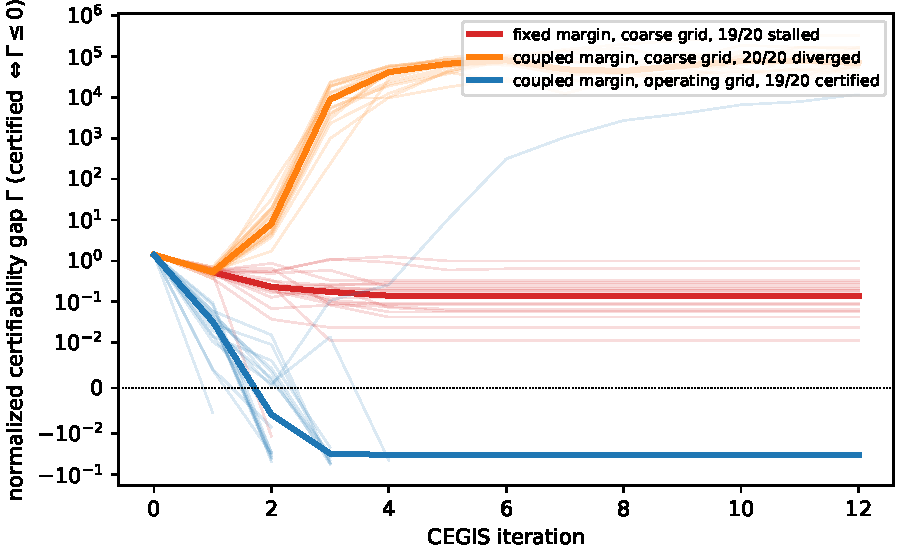
\includegraphics[width=0.72\textwidth]{fig_traces.pdf}
\caption{Certifiability gap per CEGIS iteration for three loop variants on the benchmark \eqref{eq:bench}. The fixed-margin learner stalls (Lemma~\ref{lem:stall}); the unnormalized margin-coupled learner chases scale without progress (Lemma~\ref{lem:scale}, Corollary~\ref{cor:chase}); the normalized margin-coupled learner of Algorithm~\ref{alg:cegis} certifies in one retraining round.}
\label{fig:traces}
\end{figure}

\begin{figure}[t]
\centering
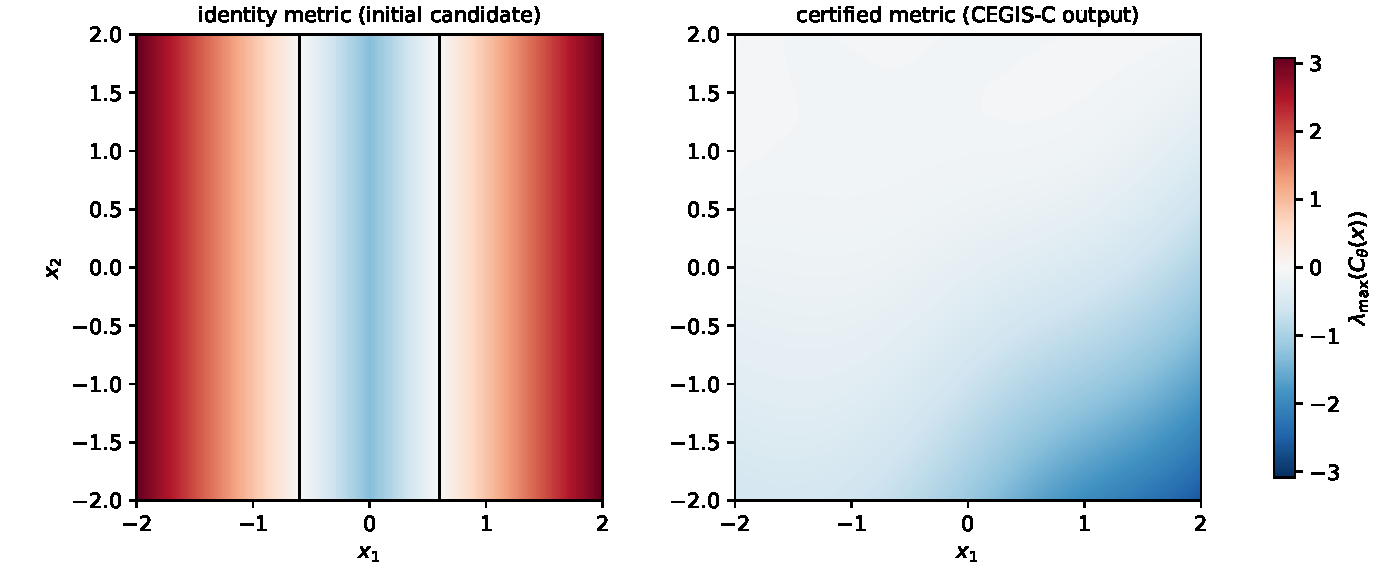
\includegraphics[width=0.95\textwidth]{fig_heatmaps.pdf}
\caption{$\lmax(C_\theta(x))$ over $\X$ for the initial identity-scaled candidate (left, zero contour in black at $|x_1| = 0.6$) and the certified CEGIS-C output (right, uniformly negative).}
\label{fig:heatmaps}
\end{figure}

\subsection{The cost of the grid oracle}

Proposition~\ref{prop:grid} certifies at resolution $\tau$ if and only if the achieved normalized slack exceeds $L_h \tau$, and by Lemma~\ref{lem:scale} the ratio $\mathrm{slack}/L_h$ is the invariant currency. Using the measured values from the certified candidate ($L_h = 0.9$, slack $0.043$), the number of grid points required on $[-2,2]^n$ scales as shown in Figure~\ref{fig:gridcost}: $3.7 \times 10^3$ points at $n = 2$, $5.3 \times 10^7$ at $n = 4$, and $1.3 \times 10^{12}$ at $n = 6$. At a budget of $10^9$ evaluations the frontier of pure grid certification sits between $n = 4$ and $n = 5$ for this benchmark's slack-to-Lipschitz ratio. The figure quantifies, rather than laments, the central obstacle: progress beyond moderate dimension requires verification oracles whose cost is not a covering number, such as interval matrix analysis with adaptive subdivision \cite{anonymous2026} or satisfiability-based encodings of the matrix inequality.

\begin{figure}[t]
\centering
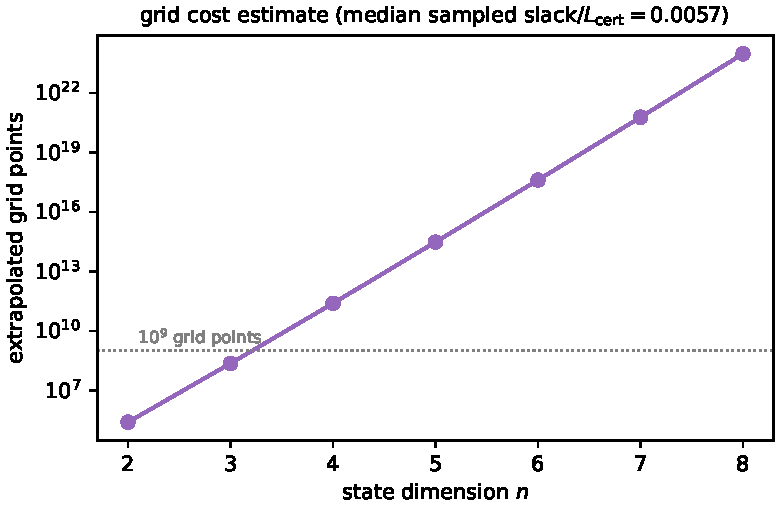
\includegraphics[width=0.58\textwidth]{fig_gridcost.pdf}
\caption{Grid points required for certification on $[-2,2]^n$ as a function of state dimension, computed from the measured slack-to-Lipschitz ratio of the certified candidate. The dotted line marks $10^9$ points.}
\label{fig:gridcost}
\end{figure}

\section{Conclusion}
\label{sec:conclusion}

We closed the counterexample-guided synthesis loop for contraction metrics and showed that the closure has theoretical content of its own. The homogeneity of the contraction condition makes certifiability a property of metric shape alone, which renders naive margin-driven training divergent and makes normalization a necessity (Lemma~\ref{lem:scale}); fixed-margin training admits non-certified fixed points (Lemma~\ref{lem:stall}); and the verified margin the corrected loop achieves converts into improved contraction rates and explicit robustness to model residuals (Theorems~\ref{thm:rate} and \ref{thm:residual}), making the framework suitable for end-to-end pipelines in which the dynamics themselves are learned. The experiments confirm each phenomenon and locate the grid oracle's dimensional frontier.

Two continuations follow directly. The first is the controlled case: carrying the loop to control contraction metrics \cite{manchester2017}, where synthesis acts on the dual metric and the verified object is related to the learned object through a matrix inverse, is the subject of a sequel in preparation. The second is the oracle: replacing covering-number verification with interval and satisfiability-based engines for parametrized matrix inequalities, the direction our cost analysis identifies as the binding constraint.

\paragraph{Reproducibility.} The complete implementation, including the three loop variants and figure generation, is available at \url{https://github.com/vmpreciado/NeuroSymbolic}.


\begin{thebibliography}{99}
\small

\bibitem{lohmiller1998}
W.~Lohmiller and J.-J.~E. Slotine,
``On contraction analysis for non-linear systems,''
\emph{Automatica}, vol.~34, no.~6, pp. 683--696, 1998.

\bibitem{manchester2017}
I.~R. Manchester and J.-J.~E. Slotine,
``Control contraction metrics: Convex and intrinsic criteria for nonlinear feedback design,''
\emph{IEEE Transactions on Automatic Control}, vol.~62, no.~6, pp. 3046--3053, 2017.

\bibitem{tsukamoto2021tutorial}
H.~Tsukamoto, S.-J. Chung, and J.-J.~E. Slotine,
``Contraction theory for nonlinear stability analysis and learning-based control: A tutorial overview,''
\emph{Annual Reviews in Control}, vol.~52, pp. 135--169, 2021.

\bibitem{dawson2023}
C.~Dawson, S.~Gao, and C.~Fan,
``Safe control with learned certificates: A survey of neural Lyapunov, barrier, and contraction methods for robotics and control,''
\emph{IEEE Transactions on Robotics}, vol.~39, no.~3, pp. 1749--1767, 2023.

\bibitem{sun2021}
D.~Sun, S.~Jha, and C.~Fan,
``Learning certified control using contraction metric,''
in \emph{Proceedings of the Conference on Robot Learning (CoRL)}, PMLR vol.~155, pp. 1519--1539, 2021.

\bibitem{tsukamoto2021ncm}
H.~Tsukamoto and S.-J. Chung,
``Neural contraction metrics for robust estimation and control: A convex optimization approach,''
\emph{IEEE Control Systems Letters}, vol.~5, no.~1, pp. 211--216, 2021.

\bibitem{chang2019}
Y.-C. Chang, N.~Roohi, and S.~Gao,
``Neural Lyapunov control,''
in \emph{Advances in Neural Information Processing Systems (NeurIPS)}, 2019.

\bibitem{abate2021}
A.~Abate, D.~Ahmed, M.~Giacobbe, and A.~Peruffo,
``Formal synthesis of Lyapunov neural networks,''
\emph{IEEE Control Systems Letters}, vol.~5, no.~3, pp. 773--778, 2021.

\bibitem{edwards2024}
A.~Edwards, A.~Peruffo, and A.~Abate,
``Fossil 2.0: Formal certificate synthesis for the verification and control of dynamical models,''
in \emph{Proceedings of the ACM International Conference on Hybrid Systems: Computation and Control (HSCC)}, 2024. arXiv:2311.09793.

\bibitem{mandal2024}
U.~Mandal et al.,
``Formally verifying deep reinforcement learning controllers with Lyapunov barrier certificates,''
arXiv:2405.14058, 2024.

\bibitem{solar2006}
A.~Solar-Lezama, L.~Tancau, R.~Bodik, S.~Seshia, and V.~Saraswat,
``Combinatorial sketching for finite programs,''
in \emph{Proceedings of ASPLOS}, 2006.

\bibitem{anonymous2026}
A.~Harapanahalli, S.~Coogan, and A.~Davydov,
``Learning certified neural network controllers using contraction and interval analysis,''
arXiv:2603.28011, 2026.

\end{thebibliography}

\end{document}
